% !TEX encoding = UTF-8 Unicode
\documentclass[
11pt,
master, % тип документа
subf, % подключить и настроить пакет subfig для вложенной нумерации рисунков
href, % подключить и настроить пакет hyperref
colorlinks=true, % цветные гиперссылки
times, % шрифт Times как основной
%fixint=false % отключить прямые знаки интегралов
]{disser}
\usepackage[left=25mm, top=20mm, right=10mm, bottom=20mm]{geometry}
\usepackage[T2A]{fontenc}
\usepackage[utf8]{inputenc}
\usepackage[english,russian]{babel}
\usepackage{amsmath,amssymb,cmap} % cmap для кодировки шрифтов в pdf
\usepackage{pdfpages} % вставляем pdf файлы
\usepackage{indentfirst} % отделять первую строку раздела абзацным отступом
\usepackage{titletoc} % убираем отступ перед "Оглавление"
\usepackage{graphicx}
\usepackage{setspace}
\usepackage{verbatim} % для оформления кода
\usepackage{pdfsync} % установка соответствия документ - код
\graphicspath{{./Img/}}

\setlength\parindent{5ex} % абзацный отступ равный пяти строчным буквам основного шрифта
\pagestyle{plain} % включаем нумерацию
\setcounter{tocdepth}{2} % включать подсекции в оглавление
\linespread{1.3} % полуторный интервал


% Номера страниц снизу и по центру
\pagestyle{footcenter}
\chapterpagestyle{footcenter}

\begin{document}
	
\pagestyle{empty}
\begin{center}
	
	\noindent  Федеральное государственное бюджетное образовательное учреждение\\
	высшего профессионального образования\\
	
	Московский государственный технический университет им. Н.Э. Баумана \\
	Факультет <<Фундаментальные науки>>\bigskip\\
	
	\vfill
	
	Лабораторная работа №4\\
	по курсу «Вычислительная физика»\\
	Тема: «Интерполяция сплайнами»\\
	\textbf{Вариант 6}\\
	
	
	\vfill
	\vfill
	\begin{flushright}
		\begin{tabular}{ll}
			Выполнили: & студенты группы ФН4-72Б     \\
			& Мистрюкова Л.А., Хижик А.И.  \\
			Проверил:  & доцент, к.физ.-мат.н.       \\
			& Хасаншин Р.Х.
		\end{tabular}
	\end{flushright}
	\vfill
	\begin{center}
		Москва, $2019$
	\end{center}
	
\end{center}
\pagebreak


\pagestyle{plain}
\tableofcontents

\section{Теоретическая часть}
\subsection{Введение}
Пусть задана сетка $\{x_n, 0\leq n\leq N\}$; точки $x_n$ -- узлы сплайна. Полиномиальным сплайном $S_p(x)$ дефекта $q$ называется функция, удовлетворяющая следующим требованиям:
\begin{enumerate}
  \item $S_p(x)$ на каждом интервале $[x_{n-1}, x_n]$ является полиномом степени $p$;
  \item Эти полиномы ``склеены'' во внутренних узлах так, что сплайн остаётся непрерывным вместе со своими $p - q$ производными: $S_p^{(k)}(x_n-0) = S_p^{(k)}(x_n+0),\; 0\leq k\leq p-q,\;1\leq n\leq N-1$.
\end{enumerate}

Чаще всего ограничиваются сплайнами дефекта $q = 1$, когда разрывна лишь старшая ($p$-я) производная, а все младшие производные непрерывны. В этом случае говорят просто о сплайне степени $p$, опуская упоминание о дефекте.

Если сплайн в заданных точках совпадает с табулированной функцией, то такой сплайн называется интерполяционным.

Примеры интерполяционных сплайнов: ломаная, проведённая через заданные точки, состоит из отрезков прямых.
В узлах она непрерывна, но первая производная разрывна. Значит, это сплайн степени $p =1$ дефекта $q = 1$. Кубический интерполяционный многочлен Эрмита склеен из кубических многочленов, а в узлах непрерывен вместе с первой производной. Это сплайн степени $p = 3$ дефекта $q = 2$.

\subsection{Кубический сплайн}
В этом случае на каждом интервале интерполяционный сплайн является многочленом третьей степени. Его удобно записать в следующем виде:
\begin{equation}\label{eq1}
  S_{3n}(x) = a_n + b_n(x-x_{n-1}) + c_n(c-x_{n-1})^2 + d_n(x-x_{n-1})^3,\;\;x_{n-1}<x<x_n,\;\;1\leq n\leq N,
\end{equation}
где коэффициенты $a_n$, $b_n$, $c_n$, $d_n$ свои для каждого интервала. Эти коэффициенты определяют из условий в узлах. Очевидно, каждый многочлен (\ref{eq1}) в своем правом и левом узлах должен совпадать с табулированными значениями функции:
\begin{equation}\label{eq2}
  S_{3n}(x_{n-1}) \equiv a_n = u_{n-1},\;\;1\leq n\leq N,
\end{equation}
\begin{equation}\label{eq3}
  S_{3n}(x_n) =  a_n + b_n h_n + c_n h_n^2 + d_n h_n^3 = u_n.
\end{equation}
Число этих уравнений вдвое меньше числа неизвестных коэффициентов, поэтому для определённости задачи нужны дополнительные условия. Для их получения вычислим первую и вторую производные многочлена (\ref{eq1}):
$$S'_{3n}(x) = b_n +2c_n(x-x_{n-1}) + 3d_n(x-x_{n-1})^2,\;\;x_{n-1}<x<x_n,\;\; 1\leq n\leq N,$$
$$S''_{3n}(x) = 2c_n + 6d_n(x-x_{n-1}),\;\;x_{n-1}<x<x_n,\;\; 1\leq n\leq N,$$
потребуем гладкости сплайна во всех точках, включая узлы. Приравняв во внутреннем узле $x_n$ правые и левые пределы производных, получим
\begin{equation}\label{eq4}
  b_{n+1} = b_n + 2c_n h_n + 3d_nh_n^2,\;\;1\leq n\leq N-1;
\end{equation}
\begin{equation}\label{eq5}
  c_{n+1} = c_n + 3d_n h_n,\;\;1\leq n\leq N.
\end{equation}
Здесь введен дополнительный коэффициент $c_{N+1}$, имеющий смысл $0.5 S''_3(x_N)$. Поэтому число уравнений (\ref{eq4}) на одно больше, чем (\ref{eq5}), а общее число неизвестных коэффициентов увеличилось на единицу.

Равенства (\ref{eq2}-\ref{eq5}) образуют систему $4N-1$ уравнений для $4N+1$ неизвестных коэффициентов.

\subsubsection{Преобразование уравнений}
Приведем систему уравнений к виду, содержащему только коэффициенты $c_n$. Уравнение (\ref{eq2}) даёт нам коэффициенты $a_n$. Из уравнений (\ref{eq5}) следует
\begin{equation}\label{eq6}
  d_n = \frac{c_{n+1}-c_n}{3h_n},\;\;1\leq n\leq N.
\end{equation}
Подставим (\ref{eq6}) в (\ref{eq3}), одновременно исключив оттуда $a_n=u_{n-1}$; получим
\begin{equation}\label{eq7}
  b_n = \frac{u_n-u_{n-1}}{h_n}-\frac{h_n(c_{n+1}+2c_n)}{3},\;\;1\leq n\leq N.
\end{equation}
Исключим из (\ref{eq4}) величины $b_n$ и $b_{n+1}$ с помощью (\ref{eq7}), соответственно увеличивая во втором случае индекс на единицу, используя (\ref{eq6}) для $d_n$. Остаётся система линейных уравнений для коэффициентов $c_n$, легко приводящаяся к следующему виду:
\begin{equation}\label{eq8}
  h_{n-1}c_{n-1} + 2(h_{n-1}+h_n)c_n + h_n c_{n+1} =3\left[\frac{u_n-u_{n-1}}{h_n}-\frac{u_{n-1}-u_{n-2}}{h_{n-1}}\right],\;\;2\leq n\leq N.
\end{equation}
Это система $N-1$ уравнения для $N+1$ неизвестных коэффициентов $c_n$. Уравнения имеют трехдиагональный вид.

Кубический сплайн похож на кубический интерполяционный многочлен, поэтому следует ожидать от него точности $O(h^4)$. Если табулированы только значения функции, то дополнительные условия приходится подбирать так, чтобы не испортить этого порядка точности. Здесь возникают две различные ситуации: $u(x)$ может быть периодической либо непериодической.

\subsubsection{Периодические граничные условия}
Рассмотрим периодическую и достаточно гладкую $u(x)$, для которой отрезок $[x_0,x_N]$ является периодом. Тогда на обоих концах отрезка функция и ее производные принимают одинаковые значения: $u^{(q)}(x_0)=u^{(q)}(x_N), ~ q=0,1,\ldots$ (при этом обязательно надо проверять исходную информацию: если $u_0\neq u_n$, то данные ошибочны). Естественно также требовать от сплайна, чтобы он удовлетворял аналогичным условиям:
\begin{equation}\label{eq9}
  S^{(q)}_{31}(x_0+0) = S^{(q)}_{3N}(x_N-0),\;\;q=\overline{0, 2}.
\end{equation}
Требовать непрерывности третьей производной мы уже не можем. При $q = 0$ условие (\ref{eq9}) автоматически следует из условия интерполяции. Значения $q = 1, ~ 2$ дают два недостающих уравнения
$$b_1 = b_N + 2c_N h_N + 3d_N h_N^2,$$
$$c_1 = c_{N+1}.$$
Исключив отсюда $b_1,~ b_N, ~ d_N$ с помощью (\ref{eq6}), (\ref{eq7}), получим граничные условия в следующем виде:
\begin{equation}\label{eq10}
  (2c_1+c_2)h_1 + (c_N+2c_{N+1})h_N = 3\left[\frac{u_1-u_0}{h_1}-\frac{u_N-u_{N-1}}{h_N}\right],
\end{equation}
$$c_1-c_{N+1}=0.$$
Заметим, что первое из этих уравнений является циклическим замыканием цепочки (\ref{eq8}). Дополнив условиями (\ref{eq10}) уравнения (\ref{eq8}), получим систему $N + 1$ линейных уравнений для определения $N + 1$ коэффициентов $c_n$. Структура матрицы этой системы приведена на рис. \ref{ris:1}.

\begin{figure}[h]
  \centering
  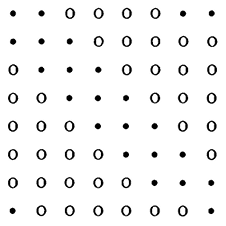
\includegraphics{Matrix.png}
  \caption{Структура матрицы для нахождения коэффициентов сплайна для периодических граничных условий}
  \label{ris:1}
\end{figure}

Эта матрица имеет ненулевые три диагонали и три угловых элемента. Соответствующая система линейных уравнений легко решается методом Гаусса без выбора главного элемента с обходом нулей, или модификацией так называемой циклической прогонки. Диагональные элементы матрицы преобладают, поэтому алгоритм очень устойчив.

Найдя коэффициенты $c_n$, оставшиеся коэффициенты сплайна вычисляют по формулам (\ref{eq2}), (\ref{eq3}) и (\ref{eq7}).

Если периодическая $u(x)$ имеет непрерывную четвертую производную, то на равномерной сетке можно получить строгую оценку погрешности:
\begin{equation}\label{eq110}
  |u(x)-S_3(x)|\leq\frac{1}{384}M_4 h^4,\;\;M_4 = \max|u^{(IV)}(x)|.
\end{equation}
Численный коэффициент в этой оценке очень мал. Точно такую же погрешность имеет локальный кубический интерполяционный многочлен Эрмита, но для его построения нужно также табулировать в узлах производные $u'_n$, а для сплайна этого не требуется. Это наглядно демонстрирует преимущество сплайна.

\subsubsection{Естественные граничные условия}
Пусть $u(x)$ непериодическая функция. Наиболее оптимальным дополнительным условием является вариационное условие. Надо минимизировать разрывы третьих производных сплайна во внутренних узлах в смысле метода наименьших квадратов. Разрыв $S_3'''(x)$ в узле $x_n$ пропорционален $d_{n+1}-d_n$. Наилучшие результаты даёт вариационное условие
\begin{equation}\label{eq112}
  \sum_{n=1}^{N-1}\frac{(d_{n+1}-d_n)^2}{h_n+h_{n+1}} = \frac{1}{3}\sum_{n=1}^{N-1}\frac{\frac{c_{n+2}-c_{n+1}}{h_{n+1}}-\frac{c_{n+1}-c_n}{h_n}}{h_n+h_{n+1}} \rightarrow \min.
\end{equation}
Условие (\ref{eq112}) вместе с уравнениями (\ref{eq8}) образует задачу на условный экстремум. Ее можно решить методом неопределённых множителей Лагранжа. Но это приводит к достаточно сложному алгоритму.

В частном случае, когда вместо всей суммы (\ref{eq112}) оставляем только крайние слагаемые c $n = l$ и $n = N - 1$, что эквивалентно требованию непрерывности $S'''_3(x)$ в приграничных узлах $x_1,\;x_{N-1}$. Это даёт $d_1=d_2$ и $d_{N-1}=d_N$. Выразив коэффициенты $d_n$ через $c_n$ по (\ref{eq6}), получим соотношения
\begin{equation}\label{eq11}
  \frac{c_2-c_1}{h_1}-\frac{c_3-c_2}{h_2}=0.
\end{equation}
$$\frac{c_{N+1}-c_N}{h_N}-\frac{c_N-c_{N-1}}{h_{N-1}}=0.$$
Соотношения (\ref{eq11}) и (\ref{eq8}) образуют систему линейных уравнений для коэффициентов $c_n$. Ее матрица отличается от трехдиагональной только первой и последней строкой, ее вид представлен на рис. \ref{ris:2}.
Такая система легко решается методом Гаусса для ленточной матрицы без выбора главного элемента, так как диагональные элементы преобладают. Этот алгоритм очень устойчив. После нахождения коэффициентов $c_n$ остальные коэффициенты выражаются через них так же, как коэффициенты периодического сплайна.
\begin{figure}[h]
  \centering
  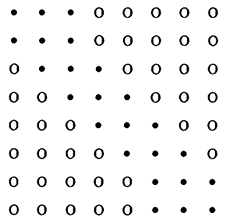
\includegraphics{Matrix2.png}
  \caption{Структура матрицы для нахождения коэффициентов сплайна для естественных граничных условий}
  \label{ris:2}
\end{figure}
Погрешность естественного сплайна есть $O(h^4)$. На некотором расстоянии от граничных интервалов при этом справедлива оценка (\ref{eq110}). Вблизи границы оценка аналогична, но с несколько большим численным коэффициентом. Этот коэффициент быстро стремится к $\frac{1}{384}$ по мере удаления от границы.

\subsection{Способы задания наклонов интерполяционного кубического сплайна}
\textbf{A.} Полагают $m_i=\frac{f_{i+1}-f_{i-1}}{2h}$, $i=\overline{1,N-1}$,
  $m_0=\frac{-3f_0+4f_1-f_2}{2h}$, $m_N=\frac{3f_N-4f_{N-1}+f_{N-2}}{2h}$.

\textbf{B.} Если известны значения $f'_i=f'(x_i)$, то полагают $m_i=f'_i$, $i=\overline{0,N}$.

\textbf{C.} Пусть $S''_3(x_i+0)$ $[S''_3(x_i-0)]$ -- значение $S''_3(x_i)$ в узле $x_i$ справа [слева], найденное из $m_i=\frac{f_{i+1}-f_{i-1}}{2h}$, $i=\overline{0,N-2}.$ Тогда
      $$S''_3(x_i+0)=-\frac{4}{h}m_i-\frac{2}{h}m_{i+1}+6\frac{f_{i+1}-f_i}{h^2},$$
      $$S''_3(x_i-0)=\frac{4}{h}m_i+\frac{2}{h}m_{i-1}-6\frac{f_i-f_{i-1}}{h^2}.$$
Потребуем непрерывность $S''_3(x)$ в узлах:
$$S''_3(x_i+0)=S''_3(x_i-0),\;\;i=\overline{1,N-1}.$$
Получим следующую систему уравнений относительно наклонов:
$$m_{i-1}+4m_i+m_{i+1}=\frac{3(f_{i+1}-f_{i-1})}{h},\;\;i=\overline{1,N-1}.$$
Для доопределения системы необходимы краевые условия. Рассмотрим некоторые из них.\\
1) Если известны $f'_0=f'(a)$ и $f'_N=f'(b)$, то задают $m_0=f'_0$ и $m_N=f'_N$.\\
2) Производные $f'_0$  и $f'_N$ аппроксимируют формулами численного дифференцирования третьего порядка точности (без остаточных членов) и полагают
$$m_0=\frac{-11f_0+18f_1-9f_2+2f_3}{6h},$$
$$m_N=\frac{11f_N-18f_{N-1}+9f_{N-2}-2f_{N-3}}{6h}.$$
3) В некоторых случаях бывают известны значения второй производной на концах отрезка $[a,b]$, т.е. величины $f''_0=f''(a)$ и $f''_N=f''(b)$. Тогда требования $S''_3(a)=f''(a)$ и $S''_3(b)=f''(b)$ приводят к краевым условиям $$m_0=-\frac{m_1}{2}+\frac{3}{2}\frac{f_1-f_0}{h}-\frac{h}{4}f''_0,$$ $$m_N=-\frac{m_{N-1}}{2}+\frac{3}{2}\frac{f_N-f_{N-1}}{h}+\frac{h}{4}f''_N.$$

Краевые условия (1-3) можно комбинировать, т.е. в левом и правом крайних узлах выбирать их независимо.
Система уравнений относительно наклонов при всех рассмотренных краевых условиях имеет единственное решение, для нахождения которого могут быть применены методы прогонки и итераций. Решая эту систему при выбранных краевых условиях находим наклоны во всех узлах и задаём сплайн на каждом частичном отрезке $[x_i,x_{i+1}]$, $i=\overline{0,N-1}$. Построенный глобальным способом сплайн $S_3(x)$ имеет дефект не больше единицы, так как этот сплайн обладает на отрезке $[a,b]$ непрерывной второй производной $S''_3(x)$.

\subsection{Погрешность приближения сплайном}
\textbf{Утверждение}. Если $f\in C_{k+1}[a,b]$, $0\leq k\leq 3$, то интерполяционный сплайн $S_3(x)$ с наклонами заданными способами B) или C), удовлетворяет неравенству
\begin{equation}\label{eq1110}
  \max_{[x_i,x_{i+1}]}|f^{(m)}(x)-S^{(m)}_3(x)|\leq ch^{k+1-m}\max_{[a,b]}|f^{(k+1)}(x)|.
\end{equation}
где $i=\overline{0,N-1}$, $m=\overline{0,k}$, с независящая от шага $h_i$ и $f$ постоянная.

Если $k=3$, и наклоны сплайна $S_3(x)$ найдены глобальным способом, то на $[a,b]$ максимальные по модулю отклонения $S_3(x)$ от $f(x)$, $S'_3(x)$ от $f'(x)$  и $S''_3(x)$ от $f''(x)$ равны соответственно $O(h^4)$, $O(h^3)$, и $O(h^2)$. При задании наклонов способом B) имеющие в узлах скачки у $S''_3(x)$ не превышают $\frac{f_{i+1}-f_{i-1}}{h}$, $i=\overline{0,N-1}$, т.е. при $k=3$ будут порядка $O(h^2)$. Эти скачки у второй производной на графике заметить трудно.

\textbf{Замечание 1}. Для кубического сплайна $S_3(x)$, наклоны которого заданы упрощённым способом А) утверждение справедливо при $0\leq k\leq 2$.

\textbf{Замечание 2}. Если $f\in C_{k+1}(-\infty,+\infty)$, $0\leq k\leq 3$ и имеет период $b-a$, то следует положить $m_0=m_N$ и к системе уравнений относительно наклонов присоединить уравнение $m_{N-1}+4m_0+m_1=\frac{3(f_1-f_{N-1})}{h}$, отвечающее значению $i=0$. Из расширенной системы, имеющей единственное решение, находятся наклоны сплайна $S_3(x)\in C_2[a,b]$; этот сплайн продолжается с отрезка $[a,b]$ на всю ось с сохранением непрерывности второй производной. При этом справедливо (\ref{eq1110}).

На больших промежутках (при больших $N$), сплайны являются более удобным средством для аппроксимации функций, чем интерполяционные многочлены.

Кубический сплайн $S_3(x)$, наклоны которого заданы глобальным способом, дважды непрерывно дифференцируем на всем отрезке $[a,b]$, т.е. имеет непрерывную кривизну.

Точность аппроксимации функции сплайном $S_3(x)$ управляется выбором $N$, т.е. шагом $h=\frac{b-a}{N}$.

\newpage
\section{Алгоритм}
\subsection{Способ А}
\begin{enumerate}
  \item Вводим на $[a, b]$ равномерную сетку с шагом $h$: $\{t_i\}_{i = 0}^n$, где $t_i = t_0 + ih$, $t_i \in [a, b],\;i = \overline{0, n}$.
  \item Вычисляем: $\{f_i\}_{i = 0}^n$, где $f_i = f(t_i)$.
  \item Вычисляем значения наклонов интерполяционного кубического сплайна в узлах сетки:
      $$m_i = \frac{f_{i + 1} - f_{i - 1}}{2 h},\;i = \overline{1, n - 1},$$
      $$m_0 = \frac{4 f_{1} - f_2 - 3 f_0}{2 h}, ~m_N = \frac{3 f_n - 4 f_{n - 1} + f_{n - 2}}{2 h}.$$
  \item Строим на каждом частичном отрезке $[x_i,x_{i+1}], ~ i=\overline{0, n-1}$ кубический сплайн:
  \begin{align*}
  	s_i(x) &= \frac{(x_{i + 1} - x)^2 [2 (x - x_i) + h]}{h^3} f_i + \frac{(x - x_{i})^2 [2 (x _{i + 1} - x) + h]}{h^3} f_{i+1} + \\
  	&+ \frac{(x_{i + 1} - x)^2 (x - x_i) }{h^2} m_i + \frac{(x- x_i)^2 (x - x_{i+ 1})}{h^2} m_{i+1}.
  \end{align*}
\end{enumerate}



\subsection{Способ В}
\begin{enumerate}
  \item Вводим на $[a, b]$ равномерную сетку с шагом $h$: $\{t_i\}_{i = 0}^n$, где $t_i = t_0 + ih$, $t_i \in [a, b]$, $i = \overline{0, n}$.
  \item Вычисляем: $\{f_i\}_{i = 0}^n$, где $f_i = f(t_i)$.
  \item Вычисляем значения наклонов интерполяционного кубического сплайна в узлах сетки:
   $m_i = f'(x_i)$, $i = \overline{0, n}$.
  \item Строим на каждом частичном отрезке $[x_i,x_{i+1}], ~ i=\overline{0, n-1}$ кубический сплайн:
\begin{align*}
	s_i(x) &= \frac{(x_{i + 1} - x)^2 [2 (x - x_i) + h]}{h^3} f_i + \frac{(x - x_{i})^2 [2 (x _{i + 1} - x) + h]}{h^3} f_{i+1} + \\
	&+ \frac{(x_{i + 1} - x)^2 (x - x_i) }{h^2} m_i + \frac{(x- x_i)^2 (x - x_{i+ 1})}{h^2} m_{i+1}.
\end{align*}
\end{enumerate}

\newpage
\section{Постановка задачи}
\begin{itemize}
  \item Построить графики интерполяционных многочленов приближающих функцию Рунге $f(x)=\frac{1}{1+25x^2}$ на отрезке $[-1,1]$, для разного числа частичных отрезков $N=5,8,15,16$. Сравнить с результатами лаб. работы №2.
      Использовать локальные способы A) и B) задания наклонов сплайна.

\end{itemize}

\newpage
\section{Программа}

{\footnotesize
\begin{verbatim}
#include <iostream>
#include <math.h>
using namespace std;

class Spline3{
private:
    double* data_x;
    double* data_y;
    double* data_m;
    double* data_m2;
    unsigned size;
    double h;
    double left_bound, right_bound;
public:
    Spline3(double* d1, double* d2, unsigned s, double l, double r){
        size = s;
        data_x = new double[size];
        data_y = new double[size];
        data_m = new double[size];
        data_m2 = new double[size];
        left_bound = l;
        right_bound = r;

        double h = (right_bound - left_bound)/(double)((size) - 1);
        for(unsigned i = 0; i < s; i++)
            data_x[i]=d1[i];
        for(unsigned i = 0; i < s; i++)
            data_y[i]= d2[i];
        data_m[0] = (-3*data_y[0] + 4*data_y[1] - data_y[2])/(2*h);
        data_m[size - 1] = (3*data_y[size - 1] - 4*data_y[size - 2] + data_y[size - 3])/(2*h);
        for (int i = 0;i <= size - 1;i++)
            data_m2[i] = Diff_Runge(left_bound  + h * i);
        for (int i = 1;i <= size - 2;i++)
            data_m[i] = (data_y[i + 1] - data_y[i - 1]) / (2 * h);
}
    double VariantA(double x, int index);
    double VariantB(double x, int index);
    void Spline();
    double Diff_Runge(double t);
};


double Spline3::Diff_Runge(double t){return -(50.0 * t )/ pow((1.0 + 25.0 * pow(t, 2)), 2);}


double Spline3::VariantA(double x, int index){
    double h = (right_bound - left_bound)/(double)((size) - 1);
    double s1, s2, s3, s4;
    double xi = data_x[index];
    double xii = data_x[index + 1];
    s1 = (pow((xii - x), 2) * (2 * (x - xi) + h)) * data_y[index] / (double)pow(h, 3);
    s2 = (pow((x - xi), 2) * (2 * (xii - x) + h)) * data_y[index + 1] / (double)pow(h, 3);
    s3 = pow((xii - x), 2) * (x - xi) * data_m[index] / (double)pow(h, 2);
    s4 = pow((x - xi), 2) * (x - xii) * data_m[index + 1] / (double)pow(h, 2);
    return s1 + s2 + s3 + s4;
}


double Spline3::VariantB(double x, int index){
    double h = (right_bound - left_bound)/(double)((size) - 1);
    double s1, s2, s3, s4;
    double xi = data_x[index];
    double xii = data_x[index + 1];
    s1 = (pow((xii - x), 2) * (2 * (x - xi) + h)) * data_y[index] / (double)pow(h, 3);
    s2 = (pow((x - xi), 2) * (2 * (xii - x) + h)) * data_y[index + 1] / (double)pow(h, 3);
    s3 = pow((xii - x), 2) * (x - xi) * data_m2[index] / (double)pow(h, 2);
    s4 = pow((x - xi), 2) * (x - xii) * data_m2[index + 1] / (double)pow(h, 2);
    return s1 + s2 + s3 + s4;
}

void Spline3::Spline(){
    cout << "Qubic Spline: "  << endl;
    double h = (right_bound - left_bound)/(double)((size) - 1);
    cout << "Varriant A: "  << endl;
    for(int i = 0; i <= size - 2; i++){
        for(int j = 0; j <= 15; j++){
            cout << VariantA(left_bound + h * i + h / 15.0 * j, i) << ", ";
        }
    }
    cout << endl;
    cout << "Variant B: "  << endl;
    for(int i = 0; i <= size - 2; i++){
        for(int j = 0; j <= 15; j++){
            cout << VariantB(left_bound + h * i + h / 15.0 * j, i) << ", ";
        }
    }
    delete data_x;
    delete data_y;
    delete data_m;
    delete data_m2;
}


double Runge_Function(double t){return 1.0 / (1.0 + 25.0 * pow(t, 2));}

int main() {
    int n = 5;
    double left_bound = -1, right_bound = 1, dat_x[n], dat_y[n];
    for (int i = 0; i < n + 1; i++){
        dat_x[i] = left_bound + (double)i * (double)(right_bound - left_bound) / (double)(n);
        dat_y[i] = Runge_Function(dat_x[i]);
    };
    Spline3 spline(dat_x, dat_y, n + 1, left_bound, right_bound);
    spline.Spline();

    return 0;
}
\end{verbatim}
}

\newpage
\section{Результаты}
\subsection{Способ А}

\begin{figure}[h]
\begin{minipage}[h]{0.48\linewidth}
\center{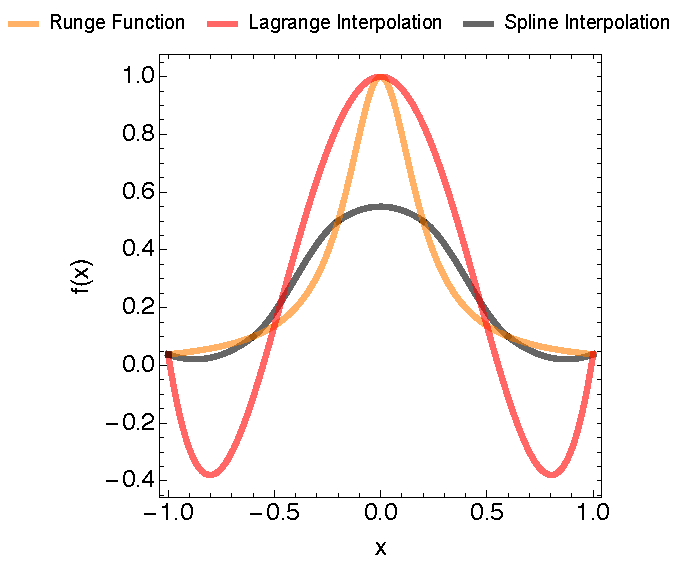
\includegraphics[width=0.8\linewidth]{N5_A}} a)
\end{minipage}
\hfill
\begin{minipage}[h]{0.48\linewidth}
\center{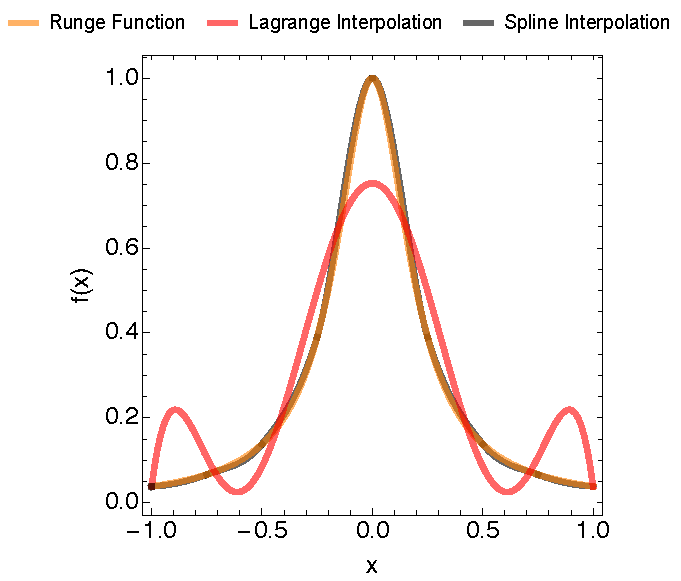
\includegraphics[width=0.8\linewidth]{N8_A}} b)
\end{minipage}
\vfill
\begin{minipage}[h]{0.48\linewidth}
\center{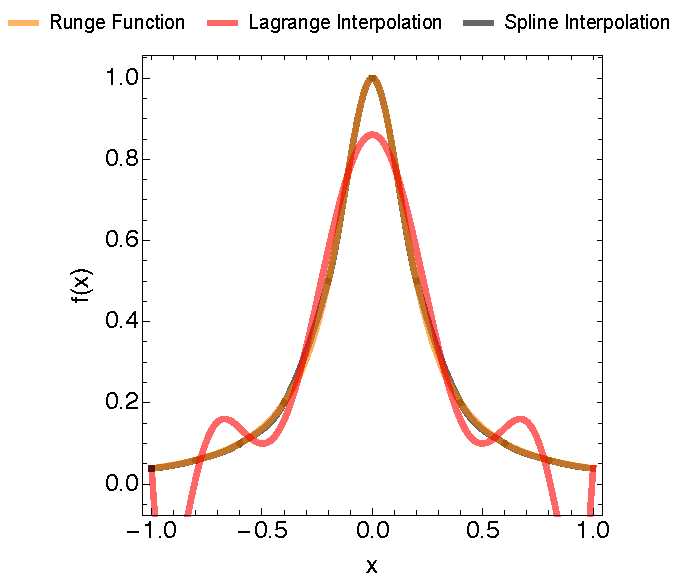
\includegraphics[width=0.8\linewidth]{N10_A}} c)
\end{minipage}
\hfill
\begin{minipage}[h]{0.48\linewidth}
\center{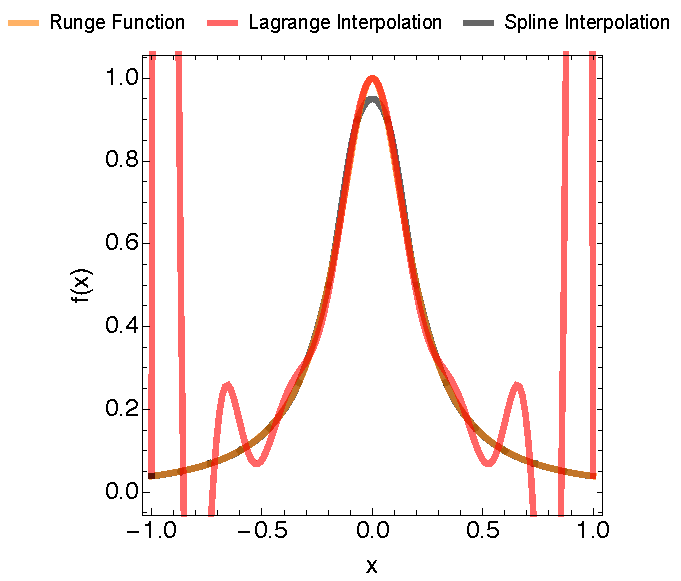
\includegraphics[width=0.8\linewidth]{N15_A}} d)
\end{minipage}
\vfill
\begin{minipage}[h]{\linewidth}
\center{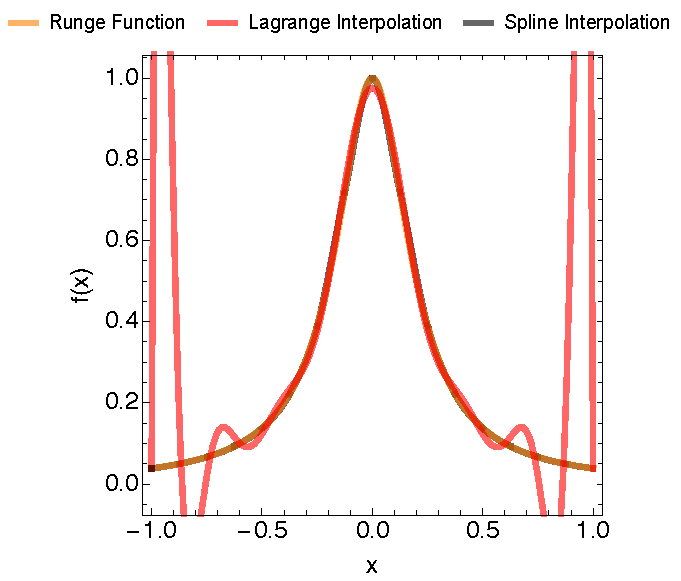
\includegraphics[width=0.38\linewidth]{N16_A}} e)
\end{minipage}
\caption{Сравнение точности интерполяция интерполяционными многочленами Лагранжа и сплайнами для a) $N=5$, b) $N=8$, c) $N=10$, d) $N=15$, e) $N=16$ частичных отрезков.}
\label{ris:3}
\end{figure}

\newpage
\subsection{Способ B}

\begin{figure}[h]
\begin{minipage}[h]{0.48\linewidth}
\center{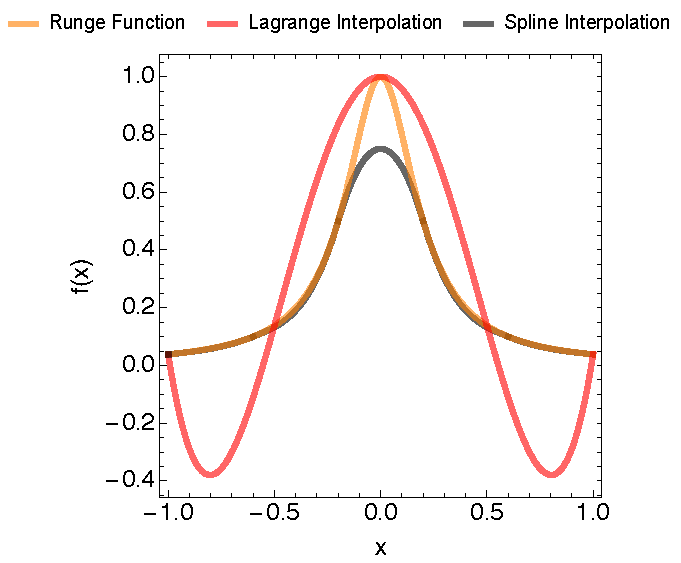
\includegraphics[width=0.8\linewidth]{N5_B}} a)
\end{minipage}
\hfill
\begin{minipage}[h]{0.48\linewidth}
\center{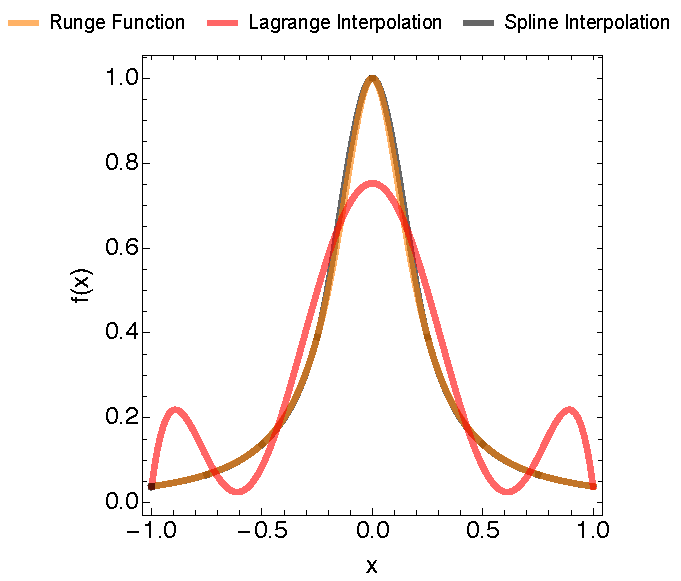
\includegraphics[width=0.8\linewidth]{N8_B}} b)
\end{minipage}
\vfill
\begin{minipage}[h]{0.48\linewidth}
\center{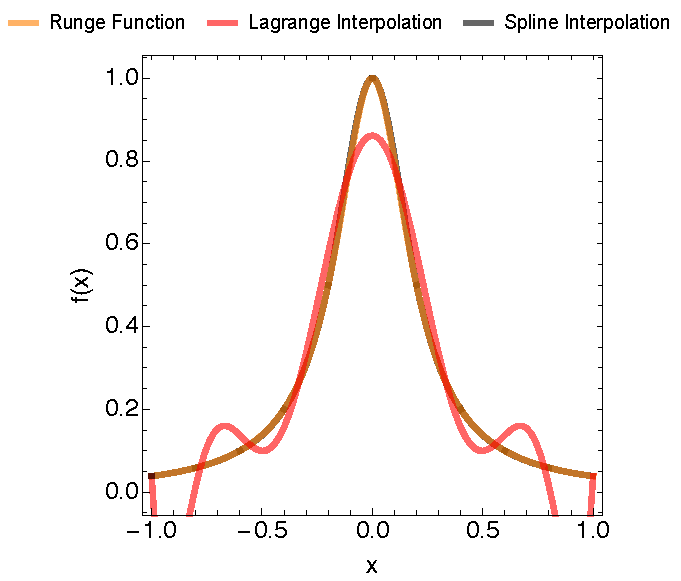
\includegraphics[width=0.8\linewidth]{N10_B}} c)
\end{minipage}
\hfill
\begin{minipage}[h]{0.48\linewidth}
\center{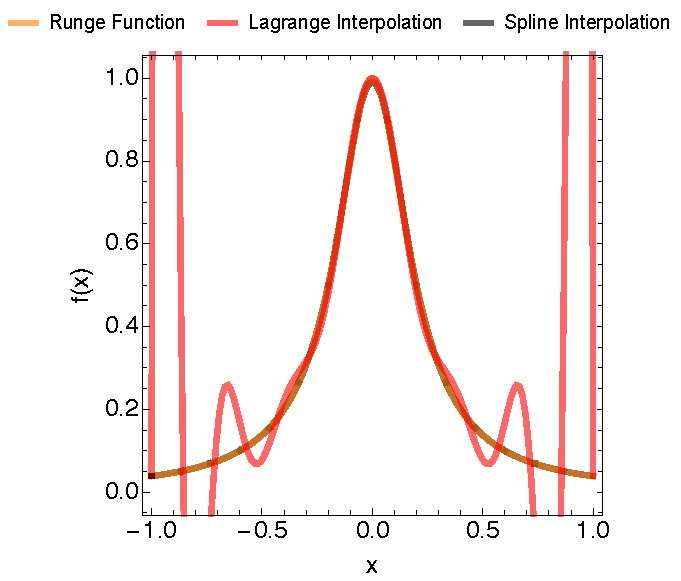
\includegraphics[width=0.8\linewidth]{N15_B}} d)
\end{minipage}
\vfill
\begin{minipage}[h]{\linewidth}
\center{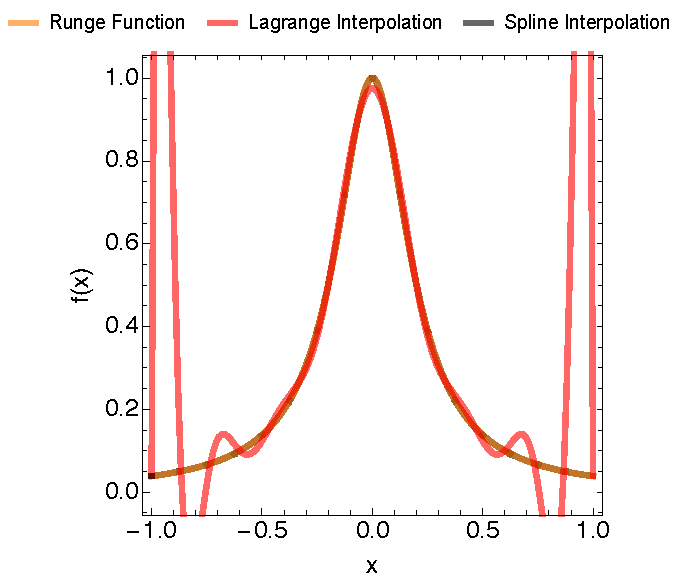
\includegraphics[width=0.38\linewidth]{N16_B}} e)
\end{minipage}
\caption{Сравнение точности интерполяция интерполяционными многочленами Лагранжа и сплайнами для a) $N=5$, b) $N=8$, c) $N=10$, d) $N=15$, e) $N=16$ частичных отрезков.}
\label{ris:4}
\end{figure}

\newpage
\section{Вывод}
Интерполяция сплайнами значительно точнее интерполяции полиномами Лагранжа, в случае сплайн-интерполяции наблюдается тенденция к уменьшения ошибки приближения с увеличением числа частичных отрезков.\\ Способ B) задания наклона сплайна показал большую точность аппроксимации, чем способ A).

\end{document} 